% ─────────────────────────────────────────────────────────────────────────────
%  Brazilian Funds Anomaly Detector — LinkedIn Carousel
%  Format: 108 × 108 mm (1080 × 1080 px @ 254 dpi)
%  Compile: pdflatex carrossel_linkedin.tex  (twice for overlays)
% ─────────────────────────────────────────────────────────────────────────────
\documentclass{beamer}

% ── Paper & margins ──────────────────────────────────────────────────────────
\usepackage{geometry}
\geometry{papersize={108mm,108mm}, margin=0mm}
\setbeamersize{text margin left=7mm, text margin right=7mm}

% ── Typography ───────────────────────────────────────────────────────────────
\usepackage[default]{lato}
\usepackage[utf8]{inputenc}
\usepackage[T1]{fontenc}
\usepackage{microtype}

% ── Links ────────────────────────────────────────────────────────────────────
\usepackage{hyperref}
\hypersetup{pdfborder={0 0 0}, colorlinks=false}

% ── Graphics / TikZ ──────────────────────────────────────────────────────────
\usepackage{tikz}
\usetikzlibrary{positioning, shadings, calc}
\usepackage{graphicx}

% ── Colour palette — mirrors the Plotly GitHub-dark theme of the charts ──────
\definecolor{BgDark}    {HTML}{0D1117}   % main background
\definecolor{BgCard}    {HTML}{161B22}   % card / chart background
\definecolor{Border}    {HTML}{30363D}   % subtle dividers
\definecolor{AccBlue}   {HTML}{58A6FF}   % primary accent
\definecolor{AccGreen}  {HTML}{3FB950}   % positive / success
\definecolor{AccOrange} {HTML}{F0883E}   % warning
\definecolor{AccRed}    {HTML}{F85149}   % danger
\definecolor{TxtPrimary}{HTML}{F0F6FC}   % headings
\definecolor{TxtSub}    {HTML}{8B949E}   % body / captions
\definecolor{TxtMuted}  {HTML}{484F58}   % very subtle text

% ── Suppress font-size substitution warnings for small math ──────────────────
\DeclareMathSizes{6.5}{6.5}{5}{4}
\DeclareMathSizes{7.5}{7.5}{5.5}{4.5}

% ── Strip all beamer chrome ───────────────────────────────────────────────────
\setbeamertemplate{navigation symbols}{}
\setbeamertemplate{footline}{}
\setbeamertemplate{headline}{}

% ── Global defaults ───────────────────────────────────────────────────────────
\setbeamercolor{background canvas}{bg=BgDark}
\setbeamercolor{normal text}{fg=TxtPrimary}
\setbeamerfont{normal text}{family=\sfdefault}

% ── Shared background: thin AccBlue bar at the very top ──────────────────────
\setbeamertemplate{background}{%
  \begin{tikzpicture}[remember picture, overlay]
    \fill[AccBlue]
      (current page.north west)
      rectangle ([yshift=-3pt] current page.north east);
  \end{tikzpicture}%
}

% ─────────────────────────────────────────────────────────────────────────────
%  MACRO: chart slide
%  #1 title  #2 pdf-file  #3 insight (AccBlue line)  #4 caption (muted)
% ─────────────────────────────────────────────────────────────────────────────
\newcommand{\chartslide}[4]{%
  \begin{frame}
    \vspace{5mm}
    % Title + accent rule
    {\fontsize{11}{13}\selectfont\textcolor{TxtPrimary}{\textbf{#1}}}\\[2pt]
    {\color{AccBlue}\rule{18mm}{1.5pt}}\\[2pt]
    % Insight line
    {\fontsize{7.5}{9.5}\selectfont\textcolor{TxtSub}{#3}}\\[2mm]
    % Chart — fills remaining width; height constrained by aspect ratio
    \begin{center}
      \includegraphics[width=\textwidth, keepaspectratio]{#2}
    \end{center}
    \vspace{-2mm}
    {\fontsize{6.5}{8}\selectfont\textcolor{TxtMuted}{#4}}
  \end{frame}%
}

% ─────────────────────────────────────────────────────────────────────────────
\begin{document}
% ─────────────────────────────────────────────────────────────────────────────


% ═══════════════════════════════════════════════════════════════════════════
% SLIDE 1 — COVER
% ═══════════════════════════════════════════════════════════════════════════
{
\setbeamertemplate{background}{%
  \begin{tikzpicture}[remember picture, overlay]
    % Gradient background
    \shade[top color=BgDark, bottom color={BgDark!85!black}]
      (current page.north west) rectangle (current page.south east);
    % Decorative glow circle — bottom right
    \fill[AccBlue, opacity=0.06]
      ([xshift=18mm, yshift=-18mm] current page.south east) circle (40mm);
    % Decorative glow circle — top left
    \fill[AccBlue, opacity=0.04]
      ([xshift=-10mm, yshift=10mm] current page.north west) circle (25mm);
    % Accent bar
    \fill[AccBlue]
      (current page.north west)
      rectangle ([yshift=-3pt] current page.north east);
    % Vertical accent stripe on the left
    \fill[AccBlue, opacity=0.15]
      (current page.north west) rectangle
      ([xshift=3pt] current page.south west);
  \end{tikzpicture}%
}
\begin{frame}
  \hspace{7mm}
  \begin{minipage}{87mm}
    \vspace{9mm}

    % Tag pill
    
\begin{tikzpicture}[baseline=(n.base)]
      \node[fill=AccBlue!12!BgDark, draw=AccBlue!40!BgDark,
            rounded corners=3pt, inner xsep=5pt, inner ysep=2.5pt] (n)
        {\fontsize{6.5}{8}\selectfont
         \textcolor{AccBlue}{\textbf{ANÁLISE · JAN–ABR 2026 · PYTHON + IA}}};
    \end{tikzpicture}

    \vspace{5mm}

    % Main headline
    {\fontsize{20}{24}\selectfont
      \textcolor{TxtPrimary}{\textbf{Como um choque}}\\
      \textcolor{TxtPrimary}{\textbf{geopolítico afeta}}\\
      \textcolor{AccBlue}{\textbf{25 mil fundos?}}
    }

    \vspace{4mm}

    {\fontsize{8}{10.5}\selectfont
      \textcolor{TxtSub}{Estreito de Ormuz · Petróleo · VIX · Ibovespa}\\[1pt]
      \textcolor{TxtSub}{Z-score · Random Forest · Claude \& DeepSeek AI}
    }

    \vspace{9mm}

    % Divider
    {\color{Border}\rule{40mm}{0.5pt}}

    \vspace{4mm}

    {\fontsize{9.5}{12}\selectfont\textcolor{TxtPrimary}{\textbf{Felipe Pereira da Silva}}}\\[1pt]
    {\fontsize{7.5}{9.5}\selectfont\textcolor{TxtSub}{Capital Markets · Analytics \& Strategy}}
  \end{minipage}
\end{frame}
}


% ═══════════════════════════════════════════════════════════════════════════
% SLIDE 2 — TRÊS CHOQUES / HERO NUMBERS
% ═══════════════════════════════════════════════════════════════════════════
\begin{frame}
  \vspace{5mm}
  \hspace{7mm}
  \begin{minipage}{87mm}

    {\fontsize{11}{13}\selectfont\textcolor{TxtPrimary}{\textbf{Um estreito fechado.}}}\\
    {\fontsize{11}{13}\selectfont\textcolor{AccBlue}{\textbf{Três choques simultâneos.}}}\\[2pt]
    {\color{AccBlue}\rule{18mm}{1.5pt}}\\[3mm]

    {\fontsize{7.5}{9.5}\selectfont\textcolor{TxtSub}%
      {O fechamento do Estreito de Ormuz propagou-se ao Brasil em menos de 72h}}

    \vspace{4mm}

    \begin{tikzpicture}
      % ── Card 1: Petróleo ──
      \node[fill=BgCard, draw=Border, rounded corners=3pt,
            text width=22mm, align=center, inner sep=2.5mm] (c1) at (0,0) {
        {\fontsize{17}{20}\selectfont\textcolor{AccOrange}{\textbf{US\$126}}}\\[1.5pt]
        {\fontsize{7.5}{9}\selectfont\textcolor{TxtPrimary}{\textbf{Brent}}}\\
        {\fontsize{6}{7.5}\selectfont\textcolor{TxtSub}{máx. em 4 anos}}
      };
      % ── Card 2: VIX ──
      \node[fill=BgCard, draw=Border, rounded corners=3pt,
            text width=22mm, align=center, inner sep=2.5mm,
            right=2mm of c1] (c2) {
        {\fontsize{17}{20}\selectfont\textcolor{AccRed}{\textbf{VIX 30}}}\\[1.5pt]
        {\fontsize{7.5}{9}\selectfont\textcolor{TxtPrimary}{\textbf{Risco Global}}}\\
        {\fontsize{6}{7.5}\selectfont\textcolor{TxtSub}{pânico nos mercados}}
      };
      % ── Card 3: USD/BRL ──
      \node[fill=BgCard, draw=Border, rounded corners=3pt,
            text width=22mm, align=center, inner sep=2.5mm,
            right=2mm of c2] (c3) {
        {\fontsize{17}{20}\selectfont\textcolor{AccBlue}{\textbf{R\$5,74}}}\\[1.5pt]
        {\fontsize{7.5}{9}\selectfont\textcolor{TxtPrimary}{\textbf{USD/BRL}}}\\
        {\fontsize{6}{7.5}\selectfont\textcolor{TxtSub}{fuga para safe haven}}
      };
    \end{tikzpicture}

    \vspace{4mm}

    {\fontsize{7.5}{9.5}\selectfont%
      \textcolor{AccGreen}{\textbf{Resultado:} }%
      \textcolor{TxtPrimary}{mais de \textbf{3.000 fundos} com comportamento}}\\
    {\fontsize{7.5}{9.5}\selectfont\textcolor{TxtPrimary}%
      {anômalo em um único dia.}}

  \end{minipage}
\end{frame}


% ═══════════════════════════════════════════════════════════════════════════
% SLIDE 3 — TIMELINE DE ANOMALIAS
% ═══════════════════════════════════════════════════════════════════════════
\chartslide%
  {Timeline de Anomalias}%
  {chart_01_timeline.pdf}%
  {Cada pico acompanhou, com 1--3 dias de defasagem, um evento do conflito Irã-EUA}%
  {Em março, mais de 10\% dos fundos brasileiros operavam fora do padrão histórico simultaneamente.}


% ═══════════════════════════════════════════════════════════════════════════
% SLIDE 4 — CHOQUE MACRO VS FUNDOS
% ═══════════════════════════════════════════════════════════════════════════
\chartslide%
  {Choque Macro vs.\ Anomalias}%
  {chart_02_market.pdf}%
  {VIX acima de 25 triplicou a densidade de anomalias — correlação de +0,32 confirmada}%
  {Linha pontilhada (eixo direito): densidade de anomalias. Ibovespa, VIX e USD/BRL no eixo esquerdo.}


% ═══════════════════════════════════════════════════════════════════════════
% SLIDE 5 — Z-SCORE
% ═══════════════════════════════════════════════════════════════════════════
\chartslide%
  {Intensidade Estatística}%
  {chart_04_zscore.pdf}%
  {Desvios extremos foram 3× mais frequentes em março-abril do que no período anterior}%
  {Azul = normal (dentro de $\pm$2,5$\sigma$). Vermelho = anomalia estatística confirmada.}


% ═══════════════════════════════════════════════════════════════════════════
% SLIDE 6 — EXPOSIÇÃO POR TIPO DE FUNDO
% ═══════════════════════════════════════════════════════════════════════════
\chartslide%
  {Exposição por Tipo de Fundo}%
  {chart_06_fundtype.pdf}%
  {FIF atingiu 38,8\% de anomalias --- multimercado absorveu o maior choque do período}%
  {FIF = maior volume (24k fundos) e primeira categoria a reagir. FI apresentou defasagem de 10+ dias.}


% ═══════════════════════════════════════════════════════════════════════════
% SLIDE 7 — O PARADOXO DO CESSAR-FOGO (hero text)
% ═══════════════════════════════════════════════════════════════════════════
\begin{frame}
  \vspace{5mm}
  \hspace{7mm}
  \begin{minipage}{87mm}

    {\fontsize{8}{10}\selectfont\textcolor{TxtSub}{\textbf{MAIOR PICO DO PERÍODO ANALISADO}}}\\[1mm]
    {\color{AccBlue}\rule{18mm}{1.5pt}}

    \vspace{4mm}

    % Big number
    {\fontsize{42}{48}\selectfont\textcolor{AccBlue}{\textbf{3.015}}}\\[-1mm]
    {\fontsize{9.5}{12}\selectfont\textcolor{TxtPrimary}{\textbf{anomalias em um único dia}}}

    \vspace{5mm}

    {\color{Border}\rule{85mm}{0.5pt}}

    \vspace{4mm}

    {\fontsize{9.5}{12}\selectfont\textcolor{AccOrange}{\textbf{Não foi durante os ataques.}}}\\[2mm]

    {\fontsize{9}{11.5}\selectfont\textcolor{TxtPrimary}%
      {Foi em \textbf{08 de abril} --- dia do cessar-fogo.}}

    \vspace{3mm}

    {\fontsize{7.5}{9.5}\selectfont\textcolor{TxtSub}%
      {O reposicionamento massivo de portfólios gerou}}\\
    {\fontsize{7.5}{9.5}\selectfont\textcolor{TxtSub}%
      {mais anomalias do que a guerra em si.}}

  \end{minipage}
\end{frame}


% ═══════════════════════════════════════════════════════════════════════════
% SLIDE 8 — VOLATILITY RATIO
% ═══════════════════════════════════════════════════════════════════════════
\chartslide%
  {Dispersão de Volatilidade}%
  {chart_05_volratio.pdf}%
  {Razão vol.\ curto/longo acima de 1,5: sinal antecipado de mudança de regime}%
  {Banda amarela = IQR entre fundos. Mediana ultrapassou o threshold em múltiplos eventos de março.}


% ═══════════════════════════════════════════════════════════════════════════
% SLIDE 9 — SINAIS PREDITIVOS / FEATURES
% ═══════════════════════════════════════════════════════════════════════════
\chartslide%
  {O que Antecipa as Anomalias?}%
  {chart_03_features.pdf}%
  {vol\_ratio é o preditor \#1 --- detectável antes do evento se manifestar nos retornos}%
  {Random Forest com 953k observações e 166 features. Importância relativa de cada variável preditora.}


% ═══════════════════════════════════════════════════════════════════════════
% SLIDE 10 — COMO FOI CONSTRUÍDO
% ═══════════════════════════════════════════════════════════════════════════
\begin{frame}
  \vspace{5mm}
  \hspace{7mm}
  \begin{minipage}{87mm}

    {\fontsize{11}{13}\selectfont\textcolor{TxtPrimary}{\textbf{Como foi construído}}}\\[2pt]
    {\color{AccBlue}\rule{18mm}{1.5pt}}\\[2mm]
    {\fontsize{7.5}{9.5}\selectfont\textcolor{TxtSub}{Pipeline end-to-end, 100\% open-source}}

    \vspace{4mm}

    \begin{tikzpicture}[node distance=2mm]
      % Stack of 4 cards
      \node[fill=BgCard, draw=Border, rounded corners=2.5pt,
            text width=79mm, inner xsep=4mm, inner ysep=2.5mm] (r1) {
        {\fontsize{8}{10}\selectfont\textcolor{AccBlue}{\textbf{01\ \ Coleta de Dados}}}\\[-0.5mm]
        {\fontsize{6.5}{8}\selectfont\textcolor{TxtSub}%
          {CVM (25k fundos) + Yahoo Finance (Ibovespa, VIX, USD/BRL) + BCB (CDI, Selic)}}
      };
      \node[fill=BgCard, draw=Border, rounded corners=2.5pt,
            text width=79mm, inner xsep=4mm, inner ysep=2.5mm,
            below=of r1] (r2) {
        {\fontsize{8}{10}\selectfont\textcolor{AccGreen}{\textbf{02\ \ Detecção de Anomalias}}}\\[-0.5mm]
        {\fontsize{6.5}{8}\selectfont\textcolor{TxtSub}%
          {Z-score rolling 63 dias, threshold $\pm$2,5$\sigma$ + volatility ratio (vol\_short/vol\_long)}}
      };
      \node[fill=BgCard, draw=Border, rounded corners=2.5pt,
            text width=79mm, inner xsep=4mm, inner ysep=2.5mm,
            below=of r2] (r3) {
        {\fontsize{8}{10}\selectfont\textcolor{AccOrange}{\textbf{03\ \ Modelo Preditivo}}}\\[-0.5mm]
        {\fontsize{6.5}{8}\selectfont\textcolor{TxtSub}%
          {Random Forest · 953k obs. · 166 features · TimeSeriesCV · exportado por tipo de fundo}}
      };
      \node[fill=BgCard, draw=Border, rounded corners=2.5pt,
            text width=79mm, inner xsep=4mm, inner ysep=2.5mm,
            below=of r3] (r4) {
        {\fontsize{8}{10}\selectfont\textcolor{AccBlue}{\textbf{04\ \ Insights com IA}}}\\[-0.5mm]
        {\fontsize{6.5}{8}\selectfont\textcolor{TxtSub}%
          {DeepSeek API: relatório executivo, análise geopolítica e breakdown por categoria}}
      };
    \end{tikzpicture}

  \end{minipage}
\end{frame}


% ═══════════════════════════════════════════════════════════════════════════
% SLIDE 11 — CTA FINAL
% ═══════════════════════════════════════════════════════════════════════════
{
\setbeamertemplate{background}{%
  \begin{tikzpicture}[remember picture, overlay]
    \shade[top color=AccBlue!18!BgDark, bottom color=BgDark]
      (current page.north west) rectangle (current page.south east);
    \fill[AccBlue, opacity=0.05]
      (current page.center) circle (45mm);
    \fill[AccBlue]
      (current page.north west)
      rectangle ([yshift=-3pt] current page.north east);
  \end{tikzpicture}%
}
\begin{frame}
  \begin{center}
    \vspace{7mm}

    {\fontsize{8}{10}\selectfont\textcolor{TxtSub}{\textbf{CONCLUSÃO}}}\\[5mm]

    {\fontsize{14}{17}\selectfont\textcolor{TxtPrimary}{\textbf{Monitorar o Ibovespa}}}\\
    {\fontsize{14}{17}\selectfont\textcolor{TxtPrimary}{\textbf{não é suficiente.}}}

    \vspace{4mm}

    {\color{Border}\rule{55mm}{0.5pt}}

    \vspace{4mm}

    {\fontsize{8}{10.5}\selectfont\textcolor{TxtSub}%
      {Risco sistêmico exige conectar dados macro}}\\
    {\fontsize{8}{10.5}\selectfont\textcolor{TxtSub}%
      {ao comportamento real dos fundos.}}

    \vspace{6mm}

    \href{https://github.com/espartafps/brazilian-funds-anomaly-detector}{%
      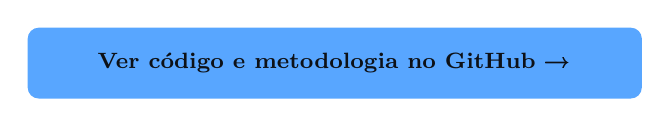
\begin{tikzpicture}
        \node[fill=AccBlue, text=BgDark,
              rounded corners=4pt,
              font=\bfseries\fontsize{8}{10}\selectfont,
              minimum width=78mm, minimum height=9mm]
          {Ver código e metodologia no GitHub\ \textrightarrow};
      \end{tikzpicture}%
    }

    \vspace{3mm}

    {\fontsize{6.5}{8}\selectfont\textcolor{TxtMuted}%
      {github.com/espartafps/brazilian-funds-anomaly-detector}}

  \end{center}
\end{frame}
}

\end{document}
